\documentclass[
  12pt,
  hidelinks,
  a4paper,
  headings=standardclasses,
  headings=big,
  spanish
]{scrartcl}

\usepackage[scale=0.8]{cascadia-code}
\usepackage[]{graphicx}
\usepackage{hyperref}
\usepackage[utf8]{inputenc}
\usepackage{csquotes}
\usepackage[T1]{fontenc}
\usepackage[spanish]{babel}
\usepackage{adjustbox}
\usepackage{bookmark}
\usepackage[]{subfigure}
\usepackage{float}
\usepackage{subcaption}
\usepackage[]{listings}
\usepackage{xcolor}

\hypersetup{
  colorlinks=true,
  linkcolor=blue,
  filecolor=magenta,
  urlcolor=blue,
  pdftitle={Proyecto Final de Base de Datos: Veterinaria},
  pdfpagemode=FullScreen,
}

\graphicspath{
  {assets}
}

\lstdefinestyle{sqlstyle}{
  language=SQL,
  extendedchars=true,
  literate={á}{{\'a}}1 {é}{{\'e}}1 {í}{{\'i}}1 {ó}{{\'o}}1 {ú}{{\'u}}1,
  basicstyle=\ttfamily\small,
  keywordstyle=\color{blue},
  stringstyle=\color{red},
  commentstyle=\color{green!50!black},
  showstringspaces=false,
  breaklines=true,
  numbers=left,
  numberstyle=\small,
  frame=single,
  backgroundcolor=\color{gray!10},
  rulecolor=\color{black}
}

\lstdefinestyle{pythonstyle}{
  language=Python,
  extendedchars=true,
  literate={á}{{\'a}}1 {é}{{\'e}}1 {í}{{\'i}}1 {ó}{{\'o}}1 {ú}{{\'u}}1,
  basicstyle=\ttfamily\small,
  keywordstyle=\color{blue},
  stringstyle=\color{red},
  commentstyle=\color{green!50!black},
  showstringspaces=false,
  breaklines=true,
  numbers=left,
  numberstyle=\small,
  frame=single,
  backgroundcolor=\color{gray!10},
  rulecolor=\color{black}
}

\begin{document}

\begin{titlepage}
  \begin{center}
    
\includegraphics[width=0.5\textwidth]{logo-upsa.png}
    \vspace*{\fill}

    \textsc{\Large{Universidad Privada de Santa Cruz de la Sierra}}\\
    \textsc{\Large{Facultad de Ingeniería}}
    \vspace*{\fill}

    \large{\textbf{Estudiante y Número de Registro:}}\\
    Jassiel Ovando Franco --- 2021117600
    \vspace*{\fill}

    \large{\textbf{Materia:}}\\
    Base de Datos --- SI~314
    \vspace*{\fill}

    \large{\textbf{Docente:}}\\
    Carlos Wilfredo Egüez Terrazas
    \vspace*{\fill}

    \large{\textbf{Proyecto:}}\\
    Grupo 2: Veterinaria
    \vspace*{\fill}

    \large{\textbf{Fecha:}}\\
    Viernes, 8 de diciembre, 2023
  \end{center}
\end{titlepage}

\newpage
{
  \hypersetup{linkcolor=black}
  \tableofcontents
  \pagebreak
  \listoffigures
}

\pagebreak
\section{Introducción}

\subsection{Enunciado para la Veterinaria}

Un veterinario tiene como pacientes: animales, y como clientes: familias.
Un cliente es un conjunto de personas que suelen corresponderse con una familia.

Cada cliente tiene: código, apellido paterno (cabeza de la familia), número de cuenta bancaria, dirección, teléfono, y nombres e identificación de personas correspondientes.
No existe el límite de personas asociadas a un cliente, además, una persona puede estar dado de alta en varios clientes.
\emph{Ejemplo: Un hombre que vive con su esposa tiene un gato y como tal pertenece a un cliente, pero también está dado de alto en el cliente asociado con el perro de sus padres.}
Los clientes pueden tener varias mascotas, cada mascota tiene: código, alias, especia, raza, color de pelo, fecha de nacimiento, peso (mantener un historial sobre el peso de la mascota por las últimas 10 visitas, además del peso actual).
Así mismo se guarda un historial médico con cada enfermedad que tuvo y la fecha en la que se enfermó.
Adicionalmente, cada mascota tiene un calendario de vacunación, en la que se llena el registro de: cada vacuna, y la enfermedad contra la que se está vacunando.

\subsubsection{Ampliación: Servicio de Hotel de Mascotas}

La veterinaria está desarrollando un nuevo negocio de \emph{hotel de mascotas}, para o cual necesitan ampliar su sistema teniendo en cuenta el funcionamiento deseado de este nuevo servicio:

\begin{itemize}
  \item Se puede hospedar a cualquier mascota sea o no paciente de la veterinaria, pero debe registrarse la información para todos.
  \item Para el huésped, debe registrarse si tiene necesidades especiales en cuanto a medicación, alimentación o algún cuidado particular.
  \item La alimentación en general se cobra como parte del servicio de hospedaje, excepto cuando requiere alimentación especial, que se factura de manera adicional, lo mismo que medicinas y otros insumos que sean necesarios para su cuidado particular.
\end{itemize}

\paragraph{Requerimientos}

\begin{enumerate}
  \item El servicio incluye también la higiene básica de un baño al ser recibido, y en estancias prolongadas un baño semanal adicional, cualquier servicio más allá de eso se considera extra en la cuenta.
  \item Se debe construir la funcionalidad necesaria para el registro de los huéspedes y todas sus necesidades.
  Además de construir la funcionalidad para la verificación (check out) del huésped y la emisión de la nota de cobranza.
  \item Se debe elaborar un reporte de los huéspedes atendidos en un periodo de entre 2 fechas, incluyendo los huéspedes que están siendo atendidos.
  \item Por último, elaborar todas las interfaces ABMC/CRUD necesarias para el manejo de los datos.
\end{enumerate}

\subsection{Consideraciones y Decisiones de Implementación}

Dado que se tiene una base para la implementación de la veterinaria, con el código ejemplar del profesor, además de el diagrama base, se hará uso del mismo donde se agregarán más elementos, tablas atributos o relaciones.
Entonces, se tendrá una base da datos (veterinaria) que almacene las siguientes tablas:
\begin{itemize}
  \item Cliente
  \item Mascota
  \item Persona
  \item Encargado
  \item Historial Médico
  \item Historial de Peso
  \item Calendario de Vacunas (más como un historial)
  \item Vacunas (para saber qué vacunas existen)
  \item Estadía (para registrar los huéspedes, para la ampliación del hotel)
  \item Requerimientos (que pedidos tienen los huéspedes)
  \item Servicios (que servicios se ofrecen en el hotel)
\end{itemize}

Cada tabla será mostrada más adelante en SQL y diagrama ERD, hecho en PlantUML y el generado por DBeaver.

Para las interfaces, se hace uso de Django, que mediante modelos, nos permite modificar, crear, eliminar, y ver los datos de la base de datos, mediante \emph{modelos}, que representan las tablas.
Aparte, el historial de pesos de mantener un registro de los 10 historiales de peso más nuevos, los viejos son descartados. Para esto se tiene un código en python que manipula la tabla en cada guardado.

Finalmente para los 2 procedimientos, \emph{el registro del huésped con generación de factura}, y \emph{el reporte de huéspedes atendidos en un periodo de 2 fechas}, se hace uso de programas de consola en python3, que se conectan a la base de datos, y realizan las consultas necesarias, para luego mostrar los datos en pantalla.

\pagebreak
\section{Modelos}

Dado que las imágenes puede que no se muestren en una buena calidad por la compresión de la imagen para que quede en el documento, el enlace al repositorio donde están las imágenes usadas es \url{https://gitlab.com/jassiel-uni/si-314/}, en el directorio \texttt{proyectos/final/doc/img}

\subsection{Modelo Conceptual}

Para el modelo conceptual no se trata de idear mucho en la parte de la ampliación, por lo tanto contiene diferencias contra los demás modelos.
Mientras que la parte base de la veterinaria, mantiene una similitud con los modelos base y demás modelos.

\begin{figure}[H]
  \centering
  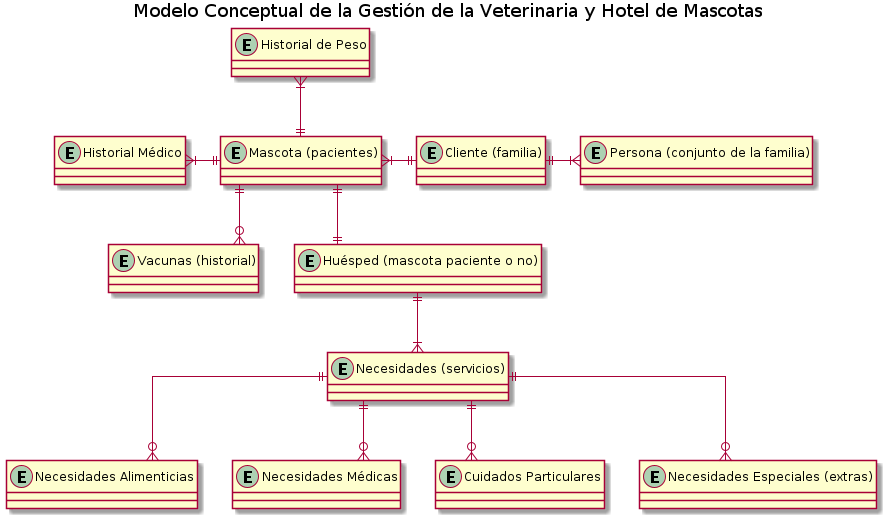
\includegraphics[width=1\textwidth]{veterinaria_modelo_conceptual.png}
  \caption{Modelo conceptual hecho en plantuml.}
\end{figure}

\pagebreak
\subsection{Modelo Lógico}
En el modelo lógico ya se procede a realizar un mejor diseño para las tablas demás de considerar las las relaciones, las llaves foráneas, tipo de atributos (entero, cadena, fecha, etc), y demás.

Se consideran nuevas tablas por parte de la ampliación para el servicio de huéspedes y sus necesidades, las cuales deberán estar en sus requerimientos dependiendo de los servicios que se ofrecen.

La tabla principal, se demuestra como la mascota, y sub-principales como el cliente y la persona, que son los que tienen más atributos y relaciones con otras tablas.

\begin{figure}[H]
  \centering
  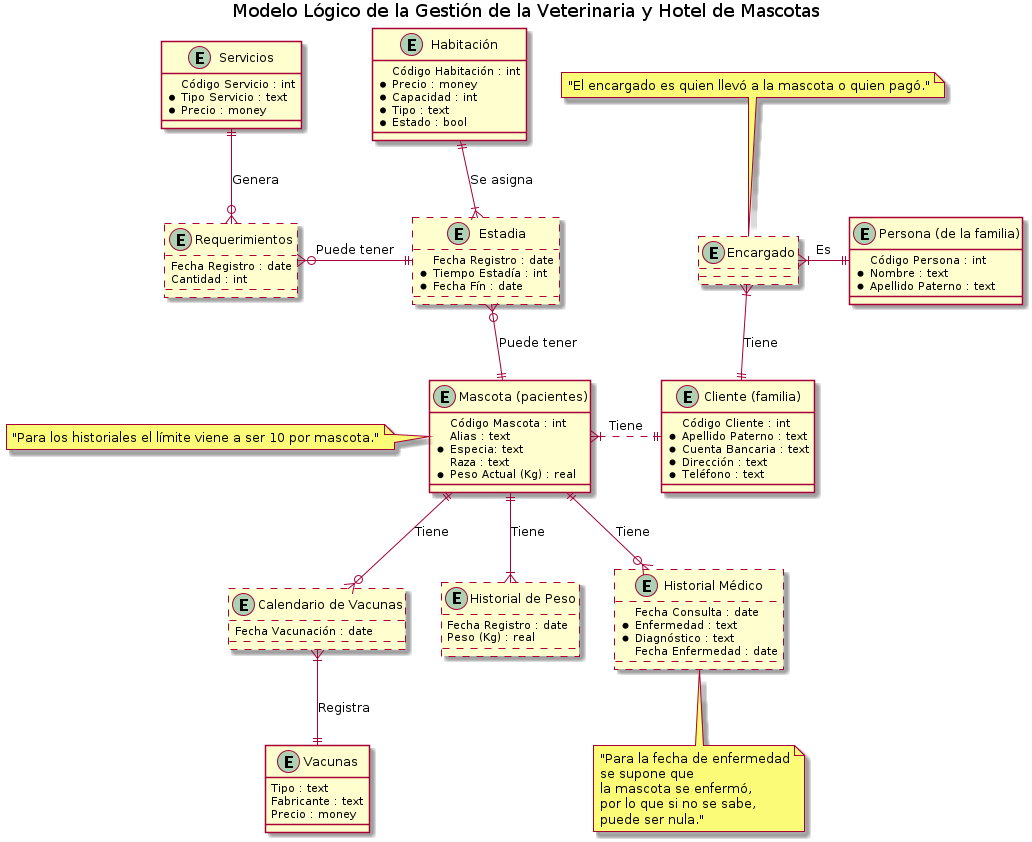
\includegraphics[width=\textwidth]{veterinaria_modelo_logico.png}
  \caption{Modelo lógico hecho en plantuml.}
\end{figure}

\pagebreak
El modelo base proporcionado por el profesor, se muestra a continuación, el cual sirve como ayuda para la creación de tablas y coherencia de un sistema mejor elaborado.

\begin{figure}[H]
  \centering
  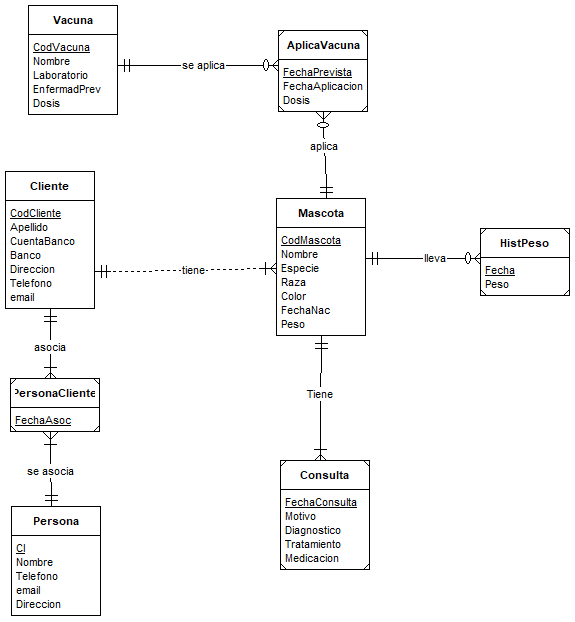
\includegraphics[width=\textwidth]{0-base.png}
  \caption{Modelo lógico proporcionado por el profesor, como base.}
\end{figure}

\pagebreak
\subsection{Modelo Físico}
Una vez se hayan hecho todas las modificaciones finales, se procede a generar el modelo físico, que está en base a la base datos ya hecha y funcional, la idea principal, prototipo se genera primeramente con PlantUML (sin haber hecho revisado la base de datos), pero luego con DBeaver y PGadmin4, se genera el modelo físico final.

\begin{figure}[H]
  \centering
  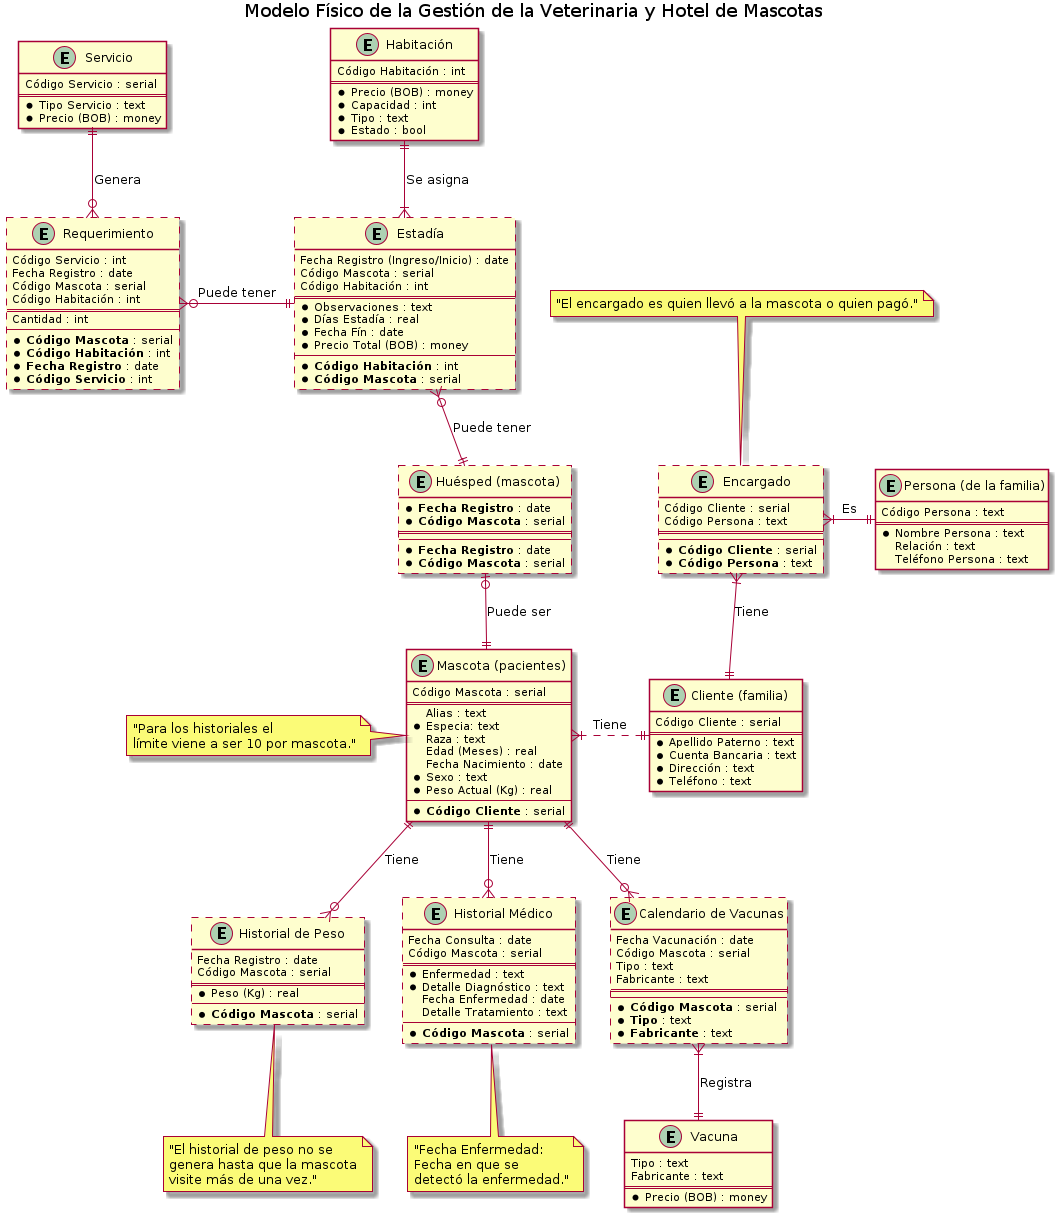
\includegraphics[width=\textwidth]{veterinaria_modelo_fisico.png}
  \caption{Modelo físico hecho en plantuml.}
\end{figure}

\subsubsection{Dbeaver}

Dbeaver proporciona un mejor modelo físico, una mejor generación y mejor detalle de las tablas, atributos, llaves primarias y foráneas, y demás.

Dado que se hace uso de django, se tienen tablas extras de autenticación con la base de datos y usuarios en la interfaz web de administración, las cuales no aparecen en ninguno de los otros modelos.

Debido a que el modelo físico es muy grande, se muestra en las siguientes páginas.

\begin{figure}[H]
  \centering
  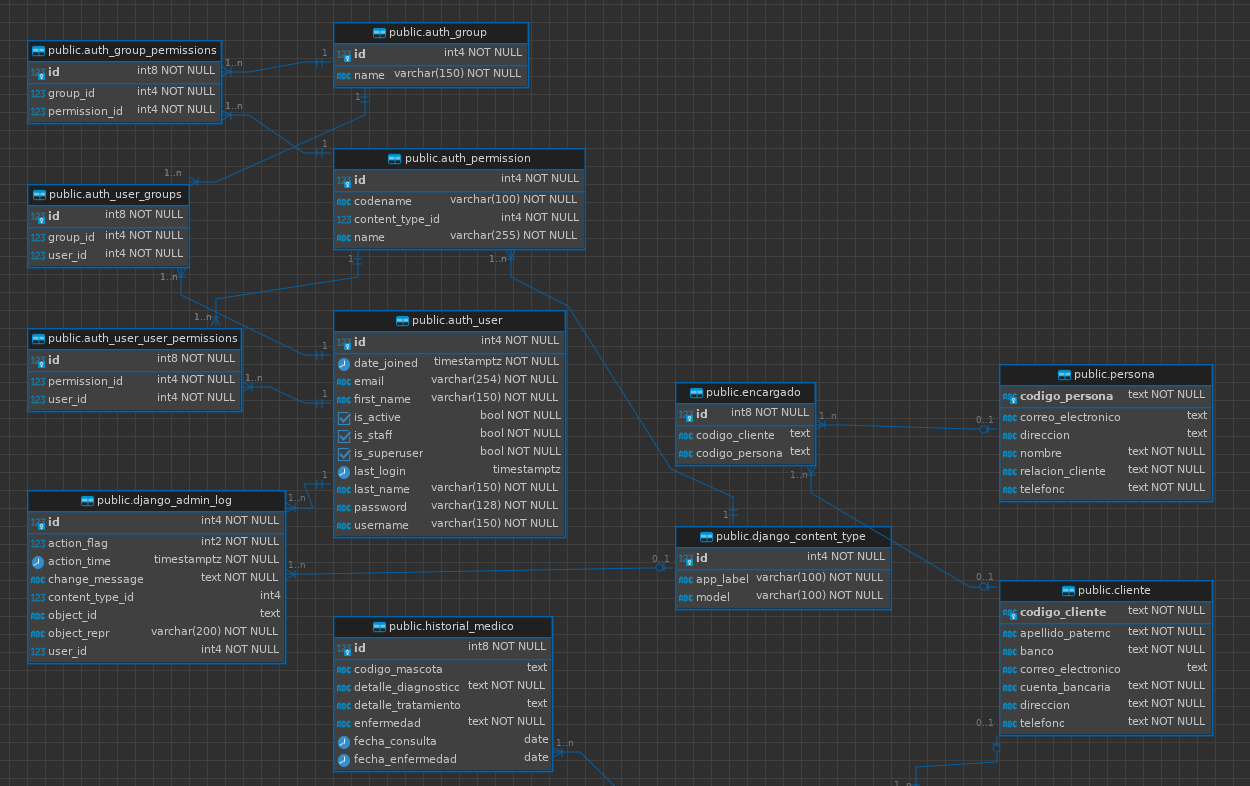
\includegraphics[width=1\textwidth]{dbeaver-1.png}
  \caption{Primera parte: Modelo físico generado por DBeaver.}
  \medskip
  \small
  Aquí se aprecia más la parte de la autenticación generada por django, y algunas tablas de (cliente y persona) de la veterinaria.
\end{figure}

\begin{figure}[H]
  \centering
  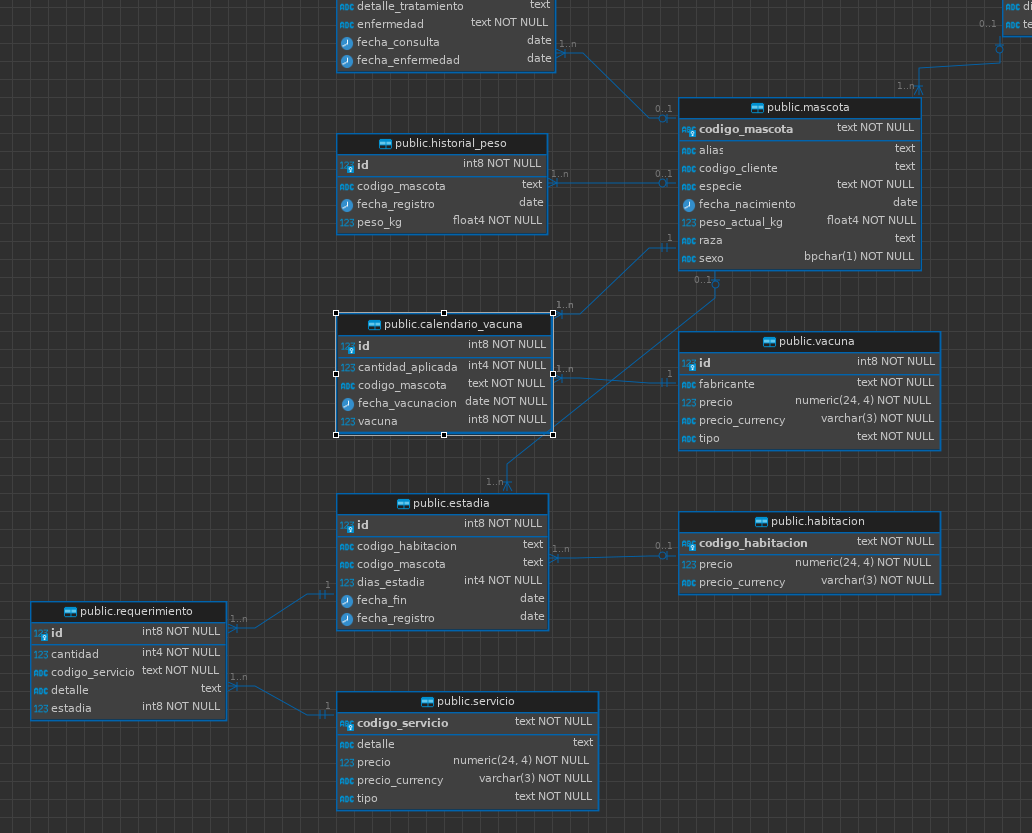
\includegraphics[width=1\textwidth]{dbeaver-2.png}
  \caption{Segunda parte: Modelo físico generado por DBeaver.}
  \medskip
  \small
  Aquí ya se puede apreciar más las tablas principales de la veterinaria, así como la ampliación para el hotel.
\end{figure}

\begin{figure}[H]
  \centering
  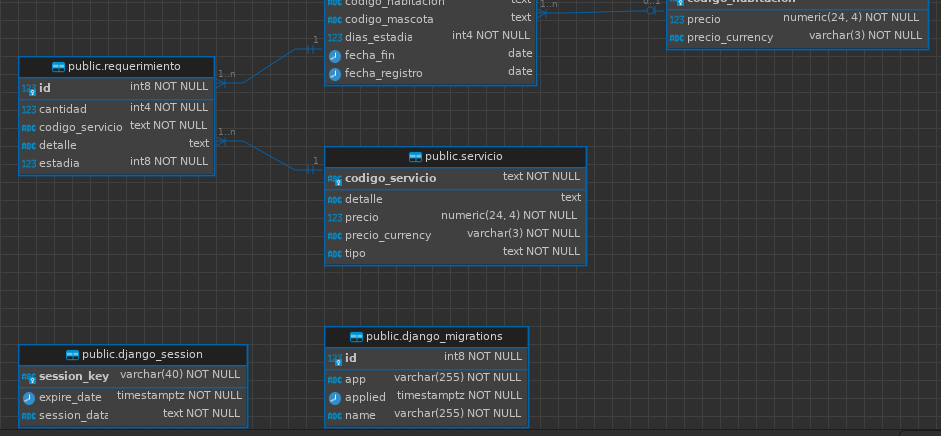
\includegraphics[width=1\textwidth]{dbeaver-3.png}
  \caption{Tercera parte: Modelo físico generado por DBeaver.}
  \medskip
  \small
  Finalmente se aprecian las tablas de migración y sesión de django más los servicios y requerimientos de la ampliación.
\end{figure}

\pagebreak
\subsubsection{PGadmin4}

PGadmin4 al igual que DBeaver, proporciona un modelo ERD, con bastantes detalles, pero dado que su generación es muy incompleta, se hace uso de DBeaver para la generación del modelo físico, principalmente. De igual forma, se procede a mostrar el modelo generado por PGadmin4.

\begin{figure}[H]
  \centering
  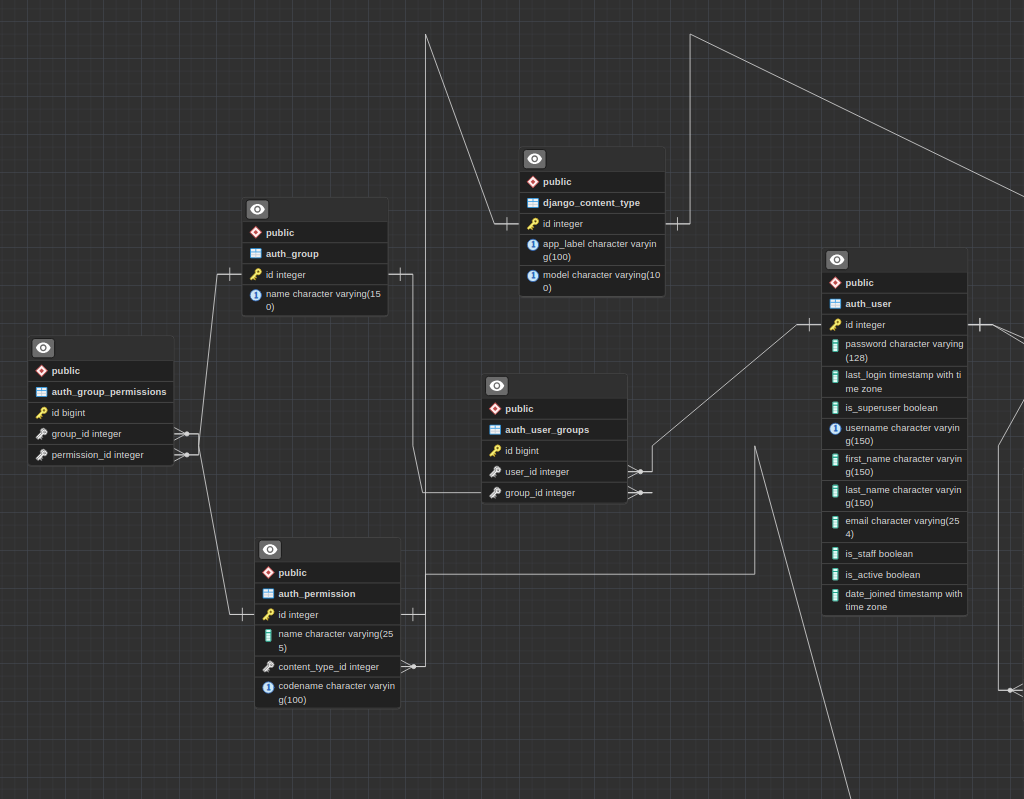
\includegraphics[width=1\textwidth]{pgadmin-1.png}
  \caption{Primera parte: Modelo físico generado por PGadmin4.}
  \medskip
  \small
  Tablas de autenticación y conexión de django.
\end{figure}

\begin{figure}[H]
  \centering
  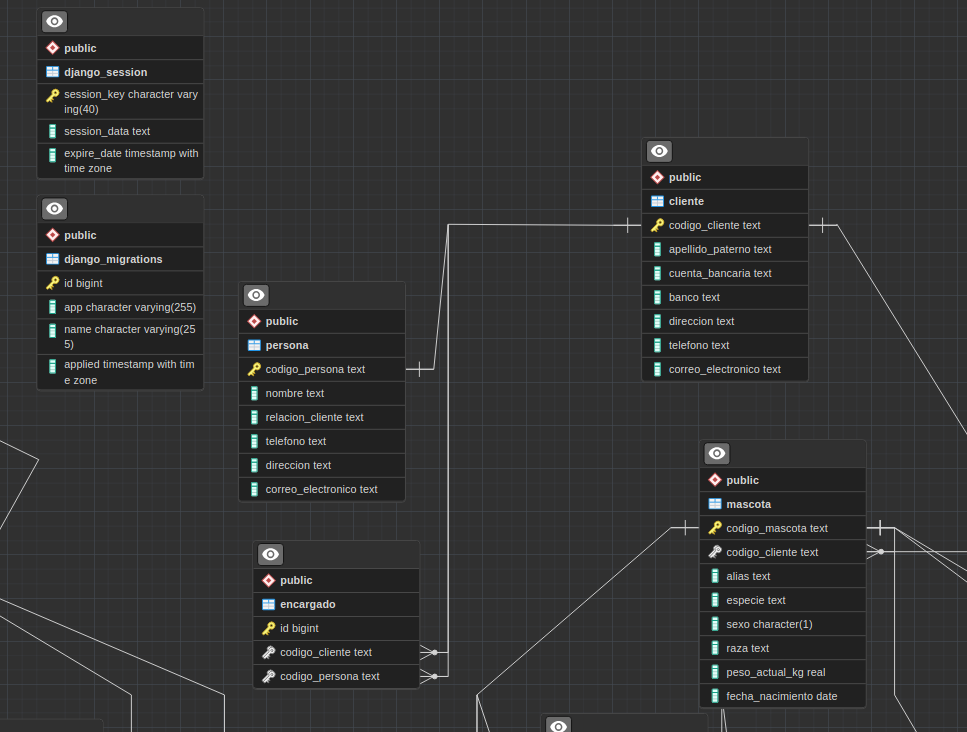
\includegraphics[width=1\textwidth]{pgadmin-2.png}
  \caption{Segunda parte: Modelo físico generado por PGadmin4.}
  \medskip
  \small
  Tablas de migración y sesión, más tablas principales de la veterinaria.
\end{figure}

\begin{figure}[H]
  \centering
  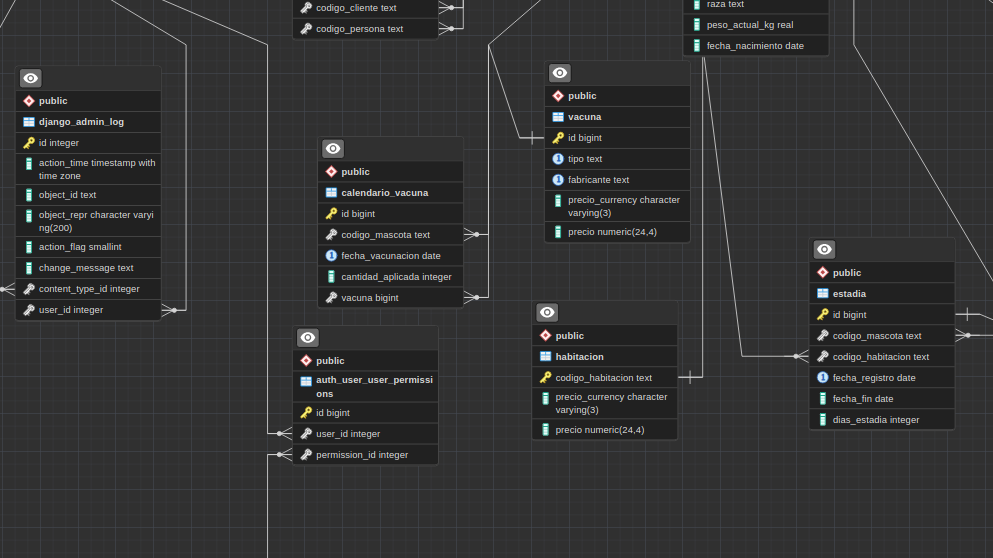
\includegraphics[width=1\textwidth]{pgadmin-3.png}
  \caption{Tercera parte: Modelo físico generado por PGadmin4.}
  \medskip
  \small
  Tablas de la ampliación del hotel.
\end{figure}

\begin{figure}[H]
  \centering
  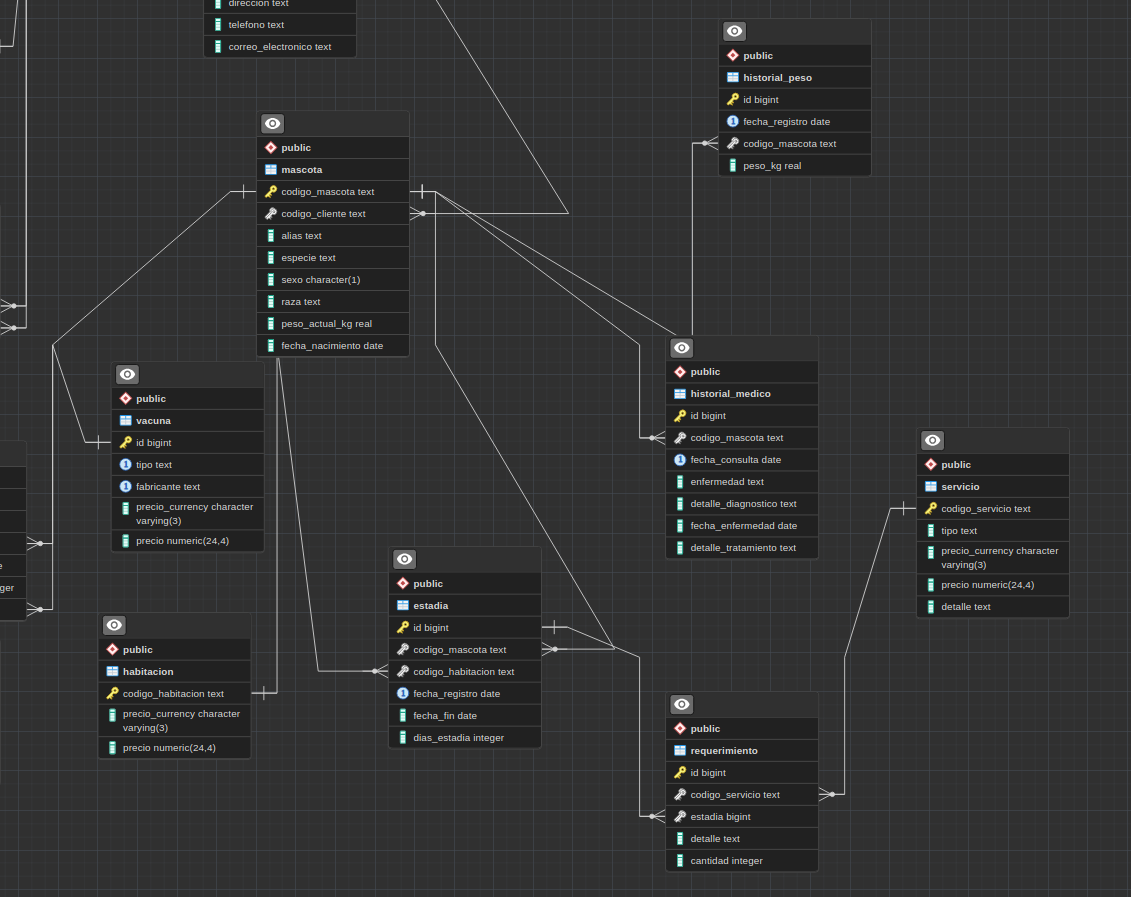
\includegraphics[width=1\textwidth]{pgadmin-4.png}
  \caption{Cuarta parte: Modelo físico generado por PGadmin4.}
  \medskip
  \small
  Ampliación e historiales bajo una vista más amplia.
\end{figure}
\pagebreak
\section{Arquitectura de la Solución Construida} % Detalles de la arquitectura empleada (cual de las arquitecturas estamos usando): dos capas, tres capas, api.

En cuanto al tipo de arquitectura que se usa, se considera una de 3 capas.

\begin{enumerate}
  \item[Primera capa:] La base de datos, que es la que almacena los datos, y se encarga de la persistencia de los mismos.
  \item[Segunda capa:] La aplicación, que es la que se encarga de la lógica de negocio, y la interacción con el usuario.
  \item[Tercera capa:] La interfaz gráfica, que es la que se encarga de la presentación de los datos, y la interacción con el usuario.
\end{enumerate}

Además de la interfaz gráfica, para las funciones extras mencionadas, como límite de historial de peso de 10 registros más nuevos, se hace uso de administración en \texttt{models.py} de django, y un código en python que se encarga de la manipulación de los datos.

Para la cobranza y \emph{check-out} de los huésped, además del reporte de huéspedes atendidos en un periodo de 2 fechas, se hace uso de programas de consola de python3, que se encarga de conectarse a la base de datos, seleccionar, las condiciones, calcular los datos, cambiarlos, y finalmente mostrarlos en pantalla.

\subsection{Herramientas Utilizadas} % Detallar lo que se puede usar y eso.

Para la base de datos, se usa netamente PostgreSQL, mediante el gestor de bases de datos DBeaver (además de PGadmin4 para ver \texttt{notices} y \texttt{logs}).
Cual nos ayuda a generar el modelo físico de la base de datos (ERC), además de usar el editor Visual Studio Code, para los archivos de código en SQL\@.
Los archivos SQL, se dividen principalmente en \texttt{ddl.sql}; donde se crean las tablas con sus atributos y llaves primarias o foráneas, \texttt{dml.sql}; donde se insertan los datos de prueba iniciales, ya que más adelante se hará uso de la interfaz gráfica para la inserción de datos, y \texttt{dql.sql}; donde se hacen las consultas a la base de datos.
Aparte de esos archivos, existe el apartado \texttt{procedimientos} donde estarán los procedimientos almacenados de la base de datos.

Para la interfaz gráfica o aplicación, se hace uso de \emph{django}, un framework de Python, que crea una aplicación web con autenticación de usuarios, más la interfaz de administración de la base de datos, configurada con postgreSQL\@.

Además de eso, como se menciona en la parte de la arquitectura, se hace uso de 2 programas en python3 que se encargan de la cobranza y reporte de periodos.

\pagebreak
\section{Implementación}

El repositorio se encuentra en \url{https://gitlab.com/jassiel-uni/si-314}, en el directorio \texttt{proyectos/final/doc/src/}, el usado en este documento, y el otro en \texttt{proyectos/final/veterinaria.sql}, para el sql sin corregir y comentarios.

\subsection{Base de Datos}
\subsubsection{Código en SQL}

Hecho en postgreSQL, si bien hay una generalización con la mayoria de codigos en \texttt{text}, se usa para poder hacer un generado automático con ayuda de django, que usa un autoguardado, por cada objeto creado, siguiendo una sintaxis con los códigos de clientes, y mascotas, principalmente.

Fuera de los códigos de cliente y mascotas, se tienen por ejemplo los códigos de habitación (números) o de servicio, que están aceptando una cantidad de texto más grande, pero se lo corrige con la interfaz de administración de django, donde solo acepta un aproximado de 5 caracteres, y se hace uso de la interfaz gráfica para la inserción de datos.

\lstinputlisting[style=sqlstyle,
  breaklines=true,
  % firstline=1,
  % lastline=10
]{../sql/ddl.sql}

\pagebreak
\subsection{Aplicación}
\subsubsection{Django --- CRUD}

\subsubsection{Cobranza}

\lstinputlisting[style=pythonstyle,
  breaklines=true,
  caption={Cobranza de huéspedes hecho en Python3.}
]{../scripts/cobranza.py}

\subsubsection{Reporte de Huéspedes entre 2 Fechas}

\lstinputlisting[style=pythonstyle,
  caption={Reporte de huéspedes entre 2 fechas hecho en Python3.}
  breaklines=true,
]{../scripts/reporte-por-periodo.py}

\pagebreak
\appendix
\section{Django}

Debido a que son 12 tablas, poner, todas las interfaces que existen, resulta en un documento muy largo, por lo tanto, se pondrán interfaces de cada tabla en diferentes etapas.

\begin{figure}[H]
  \centering
  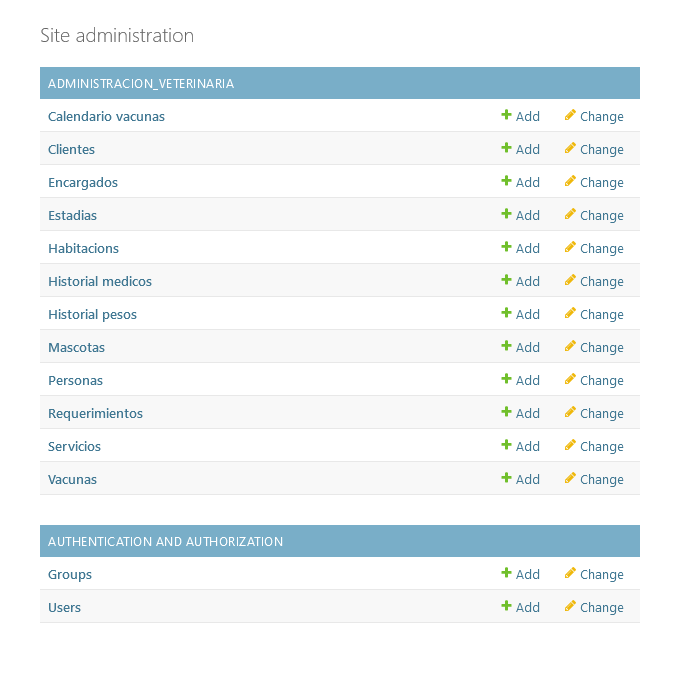
\includegraphics[width=\textwidth]{djago-menu.png}
  \caption[Menú django]{Menú de administración de django para agregar, eliminar, ver, actualizar datos.}
\end{figure}

\begin{figure}[H]
  \centering
  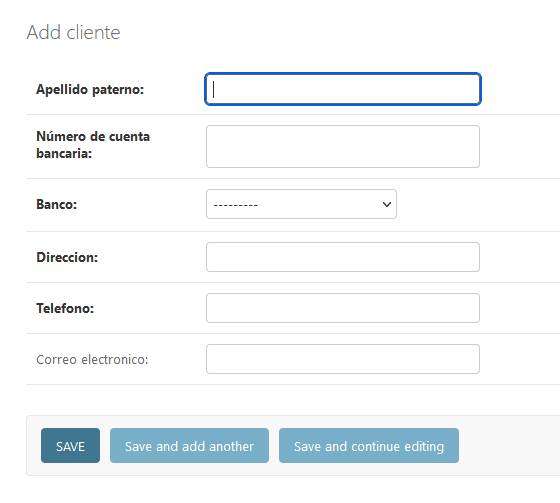
\includegraphics[width=\textwidth]{django-cliente-add.png}
  \caption{Agregar cliente en django.}
\end{figure}

\begin{figure}[H]
  \centering
  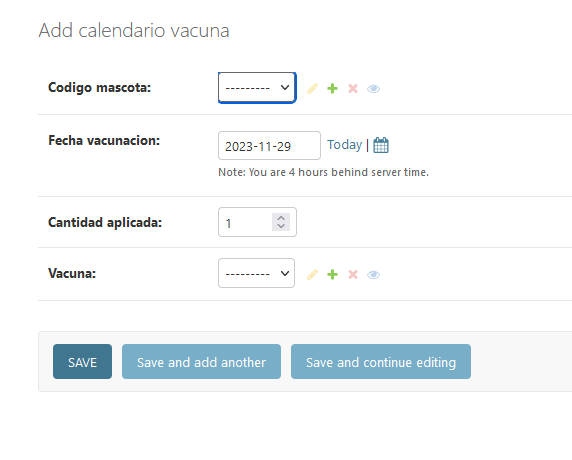
\includegraphics[width=\textwidth]{django-calendario-add.png}
  \caption{Agregar una estancia en el calendario de vacunas en django.}
\end{figure}

\begin{figure}[H]
  \centering
  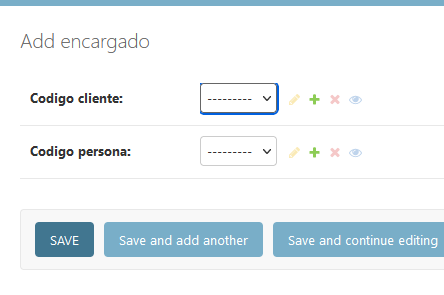
\includegraphics[width=\textwidth]{django-encargado-add.png}
  \caption{Agregar un encargado en django.}
\end{figure}

\begin{figure}[H]
  \centering
  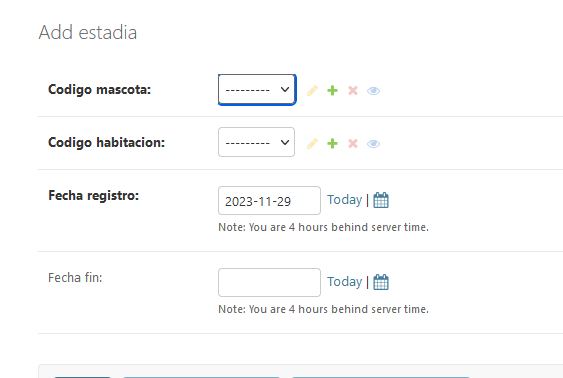
\includegraphics[width=\textwidth]{django-estadia-add.png}
  \caption{Agregar una estancia en el hotel en django.}
\end{figure}

\begin{figure}[H]
  \centering
  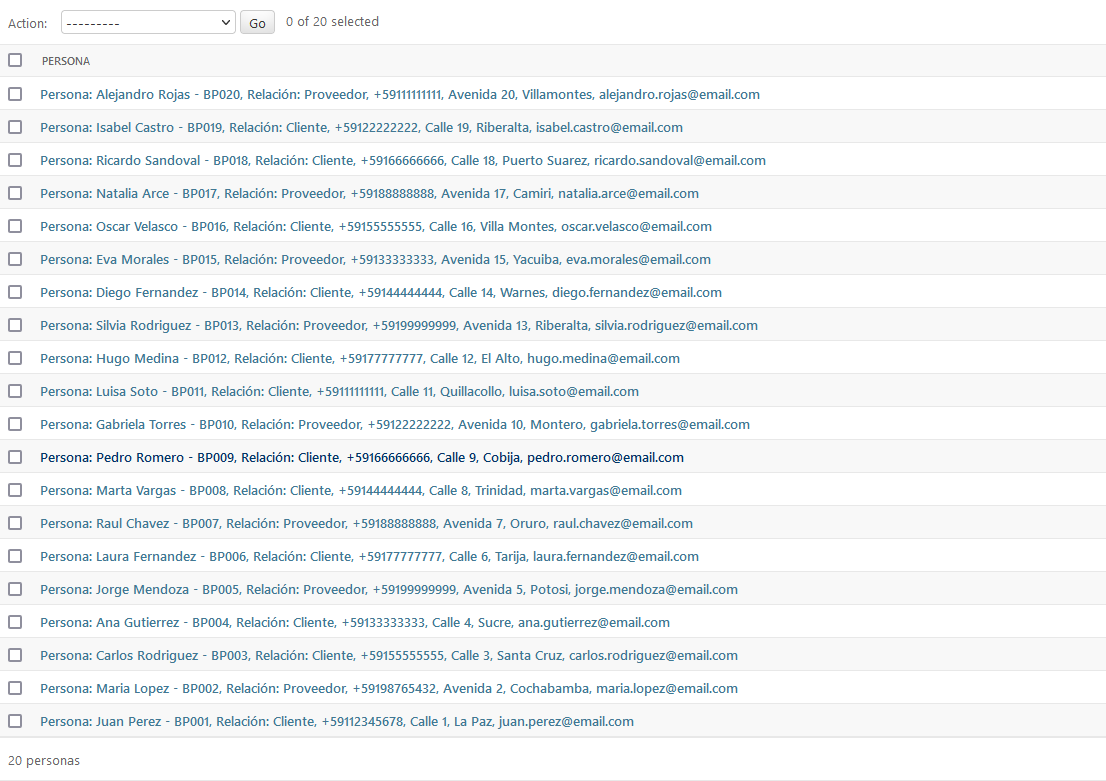
\includegraphics[width=\textwidth]{django-persona-read.png}
  \caption{Ver las personas en django.}
\end{figure}

\begin{figure}[H]
  \centering
  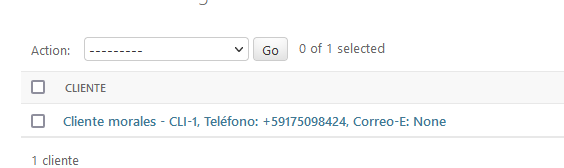
\includegraphics[width=\textwidth]{django-cliente-create.png}
  \caption{Generación de código de cliente en django (al momento de crear uno).}
\end{figure}

\begin{figure}[H]
  \centering
  \caption{Asignación de encargado en base a cliente y persona.}
  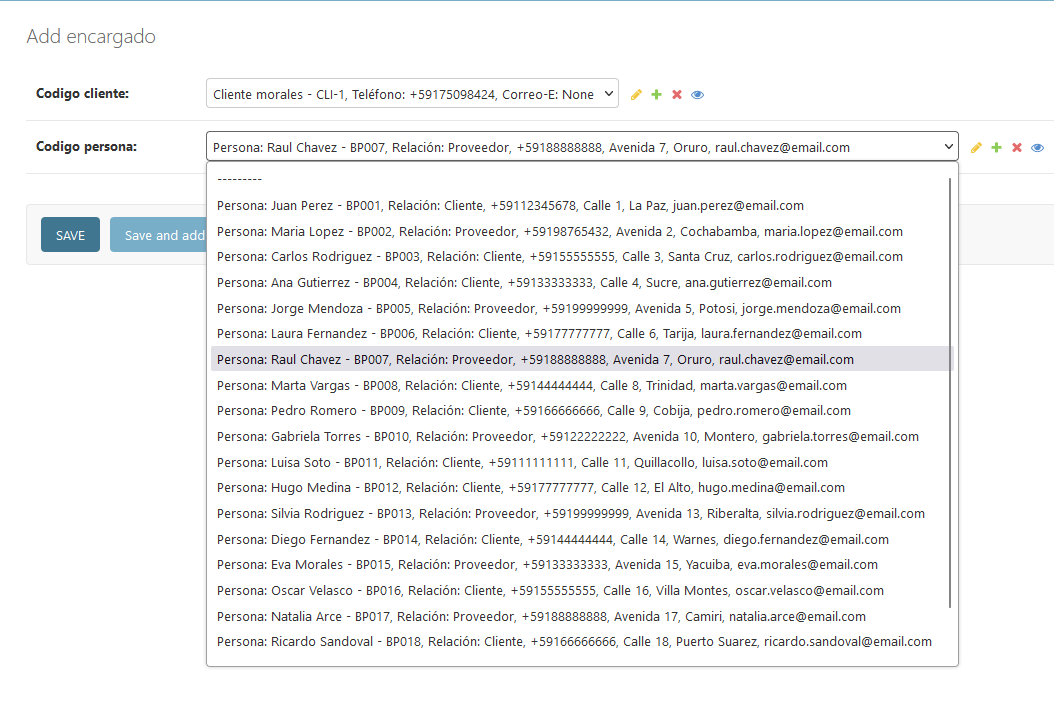
\includegraphics[width=\textwidth]{django-encargado-assign.png}
\end{figure}

\begin{figure}[H]
  \centering
  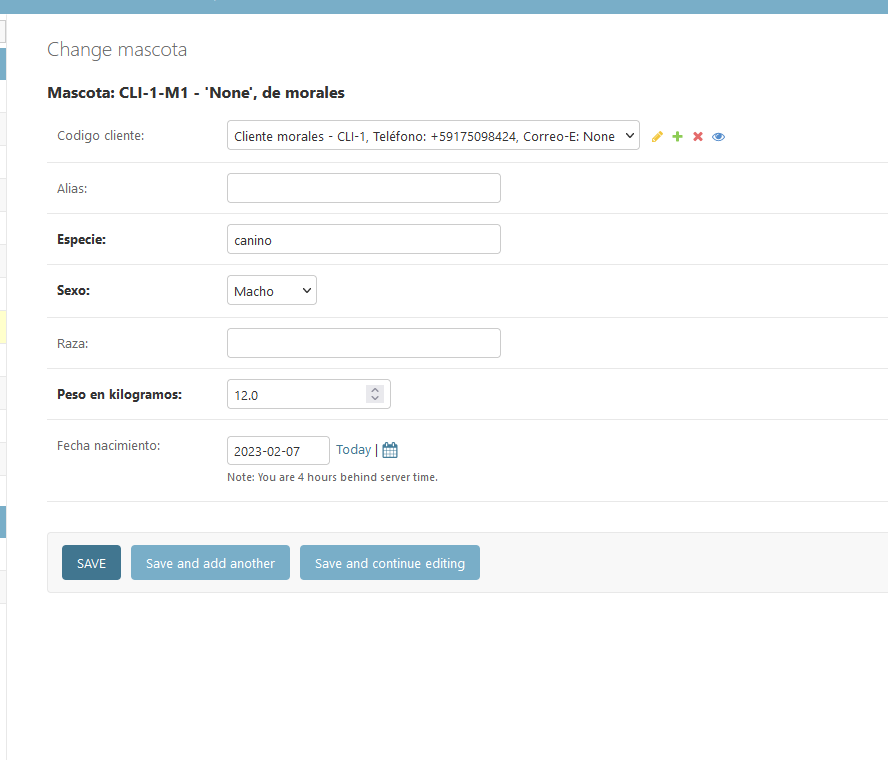
\includegraphics[width=\textwidth]{django-mascota-create.png}
  \caption{Generación de código de mascota en django (al momento de crear una).}
\end{figure}

\begin{figure}[H]
  \centering
  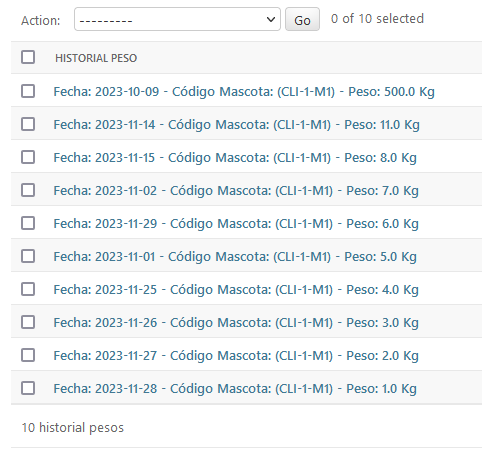
\includegraphics[width=\textwidth]{django-peso-1.png}
  \caption{10 registros de peso de mascota en django.}
  \medskip
  \small
  Comprobando que se mantiene un historial de 10 registros de peso de mascota.
  Si se agrega un nuevo registro, el más viejo es eliminado.
\end{figure}

\begin{figure}[H]
  \centering
  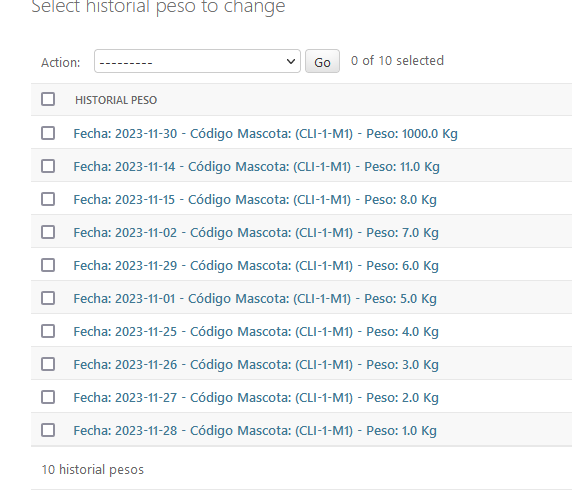
\includegraphics[width=\textwidth]{django-peso-2.png}
  \caption{10 registros de peso de mascota en django.}
  \medskip
  \small
  Comprobando que se mantiene un historial de 10 registros de peso de mascota.
  Ahora el más viejo de 500 Kg. se elimino. Esta funcionalidad se limita a la interfaz de django, si se hace por SQL, no se elimina el registro. El código será mostrada en la sección de \texttt{models.py}.
\end{figure}

\begin{figure}[H]
  \centering
  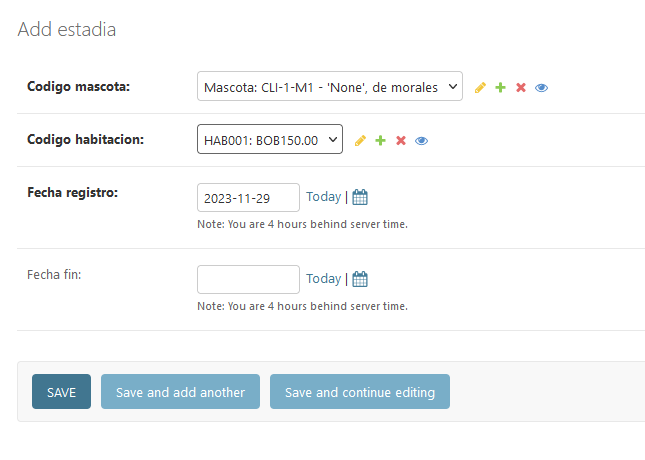
\includegraphics[width=\textwidth]{django-estancia-add.png}
  \caption{Agregar una estancia en el hotel en django.}
\end{figure}

\begin{figure}[H]
  \centering
  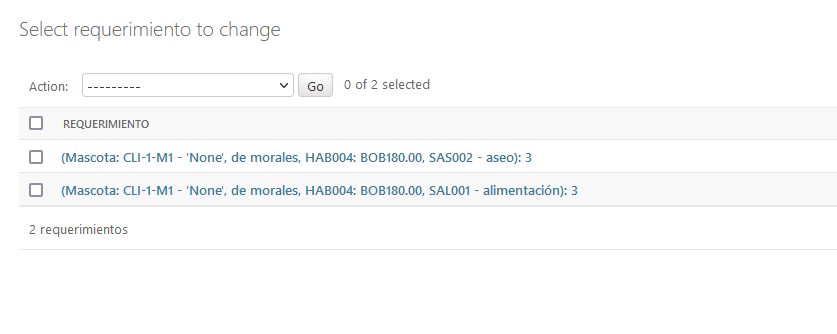
\includegraphics[width=\textwidth]{django-requisitos.add.png}
  \caption{Agregar dos requerimientos a una estadía}
\end{figure}

\pagebreak
\section{cobranza.py}

\begin{figure}[H]
  \centering
  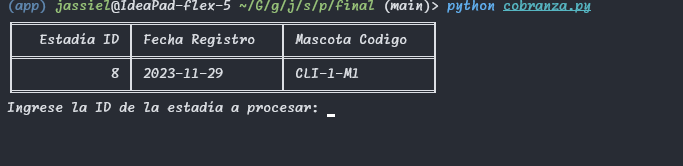
\includegraphics[width=\textwidth]{cobranza-lista.png}
  \caption{Ejecución de cobranza.py mostrando lista principal.}
\end{figure}

\begin{figure}[H]
  \centering
  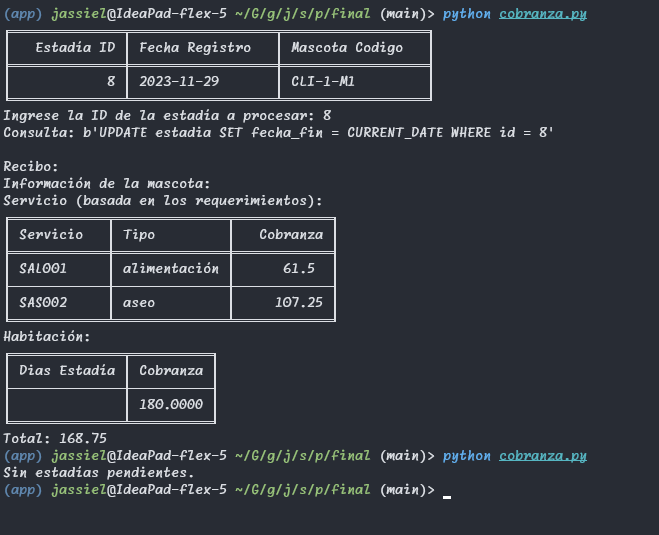
\includegraphics[width=\textwidth]{cobranza-fin.png}
  \caption{Ejecución de cobranza.py mostrando el recibo.}
\end{figure}

\begin{figure}[H]
  \centering
  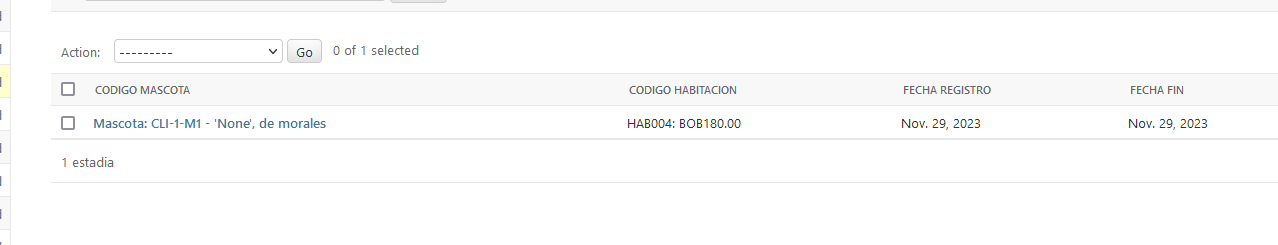
\includegraphics[width=\textwidth]{estadia-fin.png}
  \caption{Revisión en django de que se agrego la fecha.}
\end{figure}

\pagebreak
\section{reporte-por-periodo.py}

\begin{figure}[H]
  \centering
  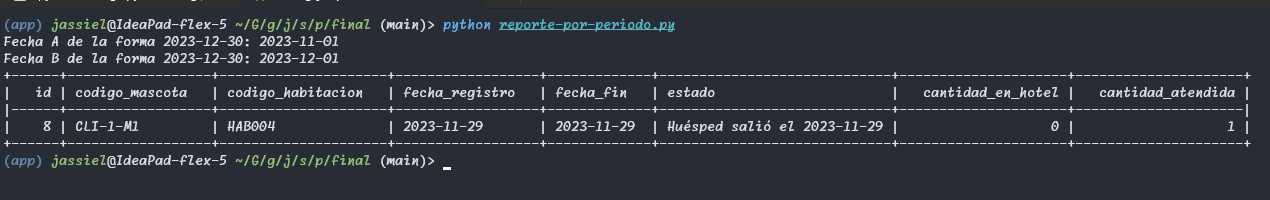
\includegraphics[width=\textwidth]{reporte-1.png}
  \caption{Ejecución de reporte-por-periodo.py mostrando la lista de huéspedes atendidos.}
\end{figure}

\pagebreak
\section{models.py}

\lstinputlisting[style=pythonstyle,
  caption={modelos para CRUD en django, en base a la base de datos.}
  breaklines=true,
]{../core/models.py}

\end{document}